%
% LaTeX template for prepartion of submissions to PLDI'15
%
% Requires temporary version of sigplanconf style file provided on
% PLDI'15 web site.
%
\documentclass[pldi]{sigplanconf-pldi15}

%
% the following standard packages may be helpful, but are not required
%

\usepackage{amsmath, amssymb}
\usepackage{mathabx}
\usepackage{mathtools}
\usepackage{wasysym}
\usepackage{stmaryrd}
%% \usepackage{SIunits}            % typset units correctly
\usepackage{courier}            % standard fixed width font
\usepackage[scaled]{helvet} % see www.ctan.org/get/macros/latex/required/psnfss/psnfss2e.pdf
\usepackage{url}                  % format URLs
\usepackage{listings}          % format code
\usepackage{enumitem}      % adjust spacing in enums
\usepackage[colorlinks=true,allcolors=blue,breaklinks,draft=false]{hyperref}   % hyperlinks, including DOIs and URLs in bibliography
% known bug: http://tex.stackexchange.com/questions/1522/pdfendlink-ended-up-in-different-nesting-level-than-pdfstartlink
\usepackage{tikz}
\usetikzlibrary{arrows.meta}
\newcommand{\doi}[1]{doi:~\href{http://dx.doi.org/#1}{\Hurl{#1}}}   % print a hyperlinked DOI
\newcommand{\scon}{\mathbin{\varstar}}
\newcommand{\ocon}{%
  \mathbin{\mbox{$\mathrlap{\cup}\hspace*{.15em}
      \raisebox{.01em}[0ex][0ex]{$\scon$}$\hspace*{.07em}}}}
\newcommand{\wand}{%
 \mathrel{\mbox{$\hspace*{-0.03em}\mathord{-}\hspace*{-0.66em}
     \mathord{-}\hspace*{-0.36em}\mathord{\scon}$\hspace*{-0.005em}}}}
\newcommand{\defeq}{\mathbin{\stackrel{\Delta}{=}}}

\begin{document}

%
% any author declaration will be ignored  when using 'plid' option (for double blind review)
%

\title{The Ramifications of Mechanizing Verification}
\authorinfo{Shengyi Wang$^{*}$ \qquad Qinxiang Cao$^{+}$ \qquad Asankhaya Sharma$^{*}$ \qquad Aquinas Hobor$^{\dagger,*}$}
{}
{School of Computing$^{*}$ and Yale-NUS College$^{\dagger}$, National University of Singapore; Princeton University$^{+}$}

\maketitle
\begin{abstract}
Blah blah blah
\end{abstract}

\newcommand\hide[1]{}

\section{Introduction}
Over the last fifteen years great strides have been made in automating verifications of programs that manipulate
tree-like data structures using separation logic CITE CITE CITE.  Unfortunately, verifying programs that manipulate
graph-like data structures (e.g. structures with \emph{intrinsic sharing}) has been far more challenging.
Indeed, verifying such programs was formidable enough that a number of the early landmark results in separation logic
devoted substantial efforts to verify single examples such as Schorr-Waite \cite{hongseok:phd} and XXX CITE with pen and
paper---avoiding entirely the additional challenges inherent in machine-assisted reasoning.

In recent years, Hobor and Villard introduced the concept of \emph{ramification} as a kind of proof pattern or framework
to verify graph-manipulating programs with pen and paper \cite{hobor:ramification}, but left open the question of how such proofs could
be incorporated in a machine-assisted setting.  In this paper, we show how this can be done, and demonstrate the
value of our approach by adding ramification to two rather sizeable---albeit quite differently flavored---separation logic-based
verification tools: the Coq-based tactic system of the Verified Software Toolchain CITE and the more highly-automated HIP/SLEEK
program verifier \cite{chin:hipsleek}.  Despite the substantial differences between these systems, the vast majority of our infrastructure is
shared between them, and since many of the other computer-assisted verification tools under development
today CITE CITE CITE CITE have much in common with at least one of these tools, we believe that our techniques will be
applicable to many other systems as well.



Along the way we discover---and show how to fix---a rather subtle error in Hobor and Villard's presentation: neither the
Knaster-Tarski \cite{tarski:fixpoint} nor the Appel-McAllester \cite{appel:fixpoint} method for solving recursive fixpoints is suitable for defining
recursive graph predicates in separation logic.

  We also develop a general framework for defining and reasoning about mathematical
graphs and

different kinds of mathematical
graphs can be implemented in separation logic in a uniform way;

generalize their setting
so that it can handle a wider variety of data structures;

We use both systems to verify a number of different programs utilizing graph-manipulating structures,
letting us understand the advantages and disadvantages of both.

\section{A framework for graph theory}
In order to verify the functional correctness of graph
algorithms, we need to first reason about mathematical graphs.
Our graph library is powerful and expressive, allowing 
us to verify realistic algorithms that work in an end-to-end
system. One of its strengths is its modularity, 
which allows us to intuitively reuse and compose our proofs when
mechanising our verifications. In this section, we present our 
mathematical graph framework with an emphasis on this modularity. 
{\color{magenta} We continue to use Union-Find from 
\S\ref{sec:orientation} as our motivating example.}

% saving old version just in case...
\hide{As will be shown in \S\ref{sec:development}, our mathematical
graph constructions comprise a considerable fraction of our
codebase. Indeed, as discussed in \S\ref{sec:related},
25 years of research into mechanized graph theory can
be summarized as ``it is a little tricky''. 
First, as demonstrated in \S\ref{sec:orientation},
our development is expressive and powerful enough to verify realistic
algorithms---that is, it actually works in an end-to-end system.
Second, we have taken considerable care to develop a modular and
general-purpose framework for such mathematical graphs to allow
such verifications to be mechanized without undue pain.
Accordingly, in this section we will present our framework
at a high level to communicate the overall architecture rather
than focusing on the nitty-gritty details.} % end hide

\subsection{Structure of the mathematical graph framework}\label{sec:mathinfra}

\begin{figure}[t]
\centering
%\beginpgfgraphicnamed{variousgraph}
\begin{tikzpicture}
[->/.style={thick,arrows={-Stealth}},
-->/.style={thick,arrows={-Stealth}, decorate, decoration={snake, amplitude=.4mm,segment length=2mm,post length=2mm}},
   realG/.style={shape=rectangle, rounded corners=4pt, draw, fill=gray!40},
   propG/.style={shape=rectangle, rounded corners=4pt, draw}]
\node[realG] (PG) at (0, 0) {\small PreGraph};
\node[realG] (LG) [right=0.8 of PG] {\small LabeledGraph};
\node[realG] (GG) [right=2 of LG] {\small GeneralGraph};
\draw [double, ->] (PG) -- (LG) node [pos=0.5, above] {\small Label} ;
\draw [double, ->] (LG) -- (GG) node (SC) [pos=0.5, above, align=center]
{\small Soundness \\ \small Condition};
\node[propG] (Prop) [below=0.6 of SC] {\small Property};
\node[propG] (PropL) [below=0.4 of Prop] {\small Property Lemmas};
\node[propG] (PGL) [below=2 of PG, align=center] {\small PreGraph \\\small Lemmas};
\node[propG] (LGL) [below=2 of LG, align=center] {\small LabeledGraph \\\small Lemmas};
\node[propG] (GGL) [below=2 of GG, align=center] {\small GeneralGraph \\\small Lemmas};
\draw [double, ->] (PGL) to (LGL);
%% \draw [double, ->] (LGL) to (GGL);
\draw [->] (PG) to (PGL);
\draw [->] (Prop) to (PropL);
\draw [-->] (Prop) to (SC);
\coordinate [left=0.2 of LG.south] (LGs1);
\coordinate [left=0.2 of LGL.north] (LGLn1);
\draw [->] (LGs1) to (LGLn1);
\coordinate [right=0.2 of LG.south] (LGs2);
\coordinate [right=0.2 of LGL.north] (LGLn2);
\draw [->] (LGs2) |- (Prop);
\draw [double, ->] (LGLn2) |- (PropL);
\coordinate [right=0.2 of GG.south] (GGs);
\coordinate [left=0.2 of GGL.north] (GGLn1);
\coordinate [right=0.2 of GGL.north] (GGLn2);
\draw [double, ->] (PropL) -| (GGLn1);
\draw [->] (GGs) to (GGLn2);
\node [draw, thick, rectangle, dashed, fit=(Prop) (PropL)] {};
\node (legend1) [below right=0.2 and -0.3 of PGL] {\small Depends};
\coordinate[left=0.8 of legend1]  (l1);
\draw [->] (l1) to (legend1);
\node (legend2) [right=1 of legend1] {\small Inherits};
\coordinate[left=0.8 of legend2]  (l2);
\draw [double, ->] (l2) to (legend2);
\node (legend3) [right=1 of legend2] {\small Instantializes};
\coordinate[left=0.8 of legend3]  (l3);
\draw [-->] (l3) to (legend3);
\end{tikzpicture}
%\endpgfgraphicnamed
\vspace{1ex}
\caption{Structure of the Mathematical Graph Library}\label{fig:graphs}
\end{figure}


Figure~\ref{fig:graphs} shows the architecture of our mathematical graph library. 
\hide{The most basic kind of graph is PreGraph, out of which we build 
LabeledGraph, and which in turn are used
to build GeneralGraphs.  Each kind has some lemmas and also inherits the lemmas of the 
previous kind.  The dashed box represents a ``plugin'' system for attaching arbitrary 
properties to LabeledGraphs (\ref{subsec:graphplugins}). %and will be discussed later. 
%We will consider each in turn.
} % end hide

\begin{figure}[t]
\centering
\beginpgfgraphicnamed{pregraphexp}
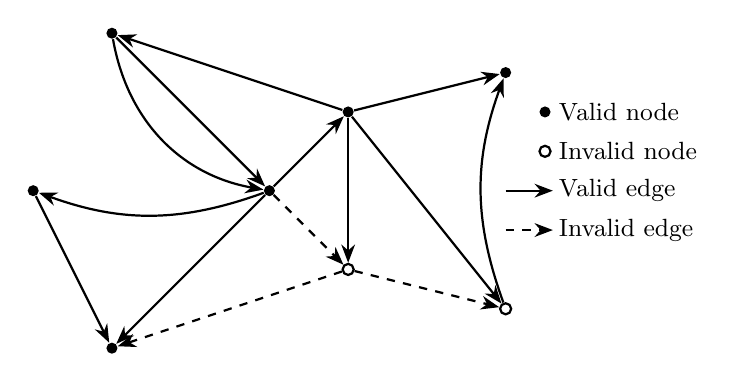
\begin{tikzpicture}
[vad/.style={circle, fill=black, inner sep=0pt, minimum size=4pt},
 inv/.style={circle, draw=black, thick, inner sep=0pt, minimum size=4pt},
 ->/.style={thick, arrows={-Stealth}}]
\node[vad] (n1) at (0, 0) {};
\node[vad] (n2) at (1, 1) {};
\node[inv] (n3) at (1, -1) {};
\node[vad] (n4) at (-2,2) {};
\node[vad] (n5) at (-2,-2) {};
\node[vad] (n6) at (-3,0) {};
\node[vad] (n7) at (3,1.5) {};
\node[inv] (n8) at (3,-1.5) {};
\node[vad] (n9) at (3.5, 1) {};
\node[inv] (n10) at (3.5, 0.5) {};
\node at (3.5, 1) [right=1.5pt] {\small Valid node};
\node at (3.5, 0.5) [right=1.5pt] {\small Invalid node};
\node at (3.5, 0) [right=1.5pt] {\small Valid edge};
\node at (3.5, -0.5) [right=1.5pt] {\small Invalid edge};
\draw[->] (n1) to (n2);
\draw[->,dashed] (n1) to (n3);
\draw[->,dashed] (n3) to (n5);
\draw[->] (n2) to (n3);
\draw[->] (n2) to (n7);
\draw[->] (n2) to (n8);
\draw[->,dashed] (n3) to (n8);
\draw[->] (n4) to (n1);
\draw[->] (n1) to (n5);
\draw[->] (n2) to (n4);
\draw[->] (n1) to [bend left=20] (n6);
\draw[->] (n6) to (n5);
\draw[->] (n8) to [bend left=20] (n7);
\draw[->] (n4) to [bend right=35] (n1);
\draw[->] (3.0, 0) -- (3.6, 0);
\draw[->,dashed] (3.0, -0.5) -- (3.6, -0.5);
\end{tikzpicture}
\endpgfgraphicnamed
\vspace{1ex}
\caption{A PreGraph with valid and invalid vertices and edges.}\label{fig:pregraph}
\end{figure}
% move to its own file?

\vspace{-0.75ex}
\iftrue
\paragraph{PreGraph.} A PreGraph is a hextuple $(VT, ET, V, E, s, d)$, where $VT$ 
and $ET$ are the underlying carrier sets of vertices and edges, and $V$ and $E$, 
subsets $VT$ and $ET$ respectively, introduce the notion of \emph{validity} in the 
graph. In Figure \ref{fig:pregraph}, valid vertices are in $V$ and 
invalid vertices are in $VE \smallsetminus V$. Importantly, 
both kinds of vertices are legally part 
of the PreGraph. Finally, $s$ and $d$ are functions that map 
an edge to its source and destination respectively; {\color{magenta}this model means 
that PreGraphs are directed rather than undirected.} 
With an eye to flexibility, we make no further 
requirements of a legal PreGraph, not even a specific notion 
of how the four sets are related.
Indeed, the PreGraph in Figure \ref{fig:pregraph} contains invalid 
vertices and edges in an arbitrary configuration.

Many graph concepts such as \emph{path}, \emph{reachability}, and \emph{subgraph} are 
defined on PreGraphs. In \S\ref{fig:find} we saw \emph{reachable}, written 
$\m{a} \mathrel{{\stackrel{\gamma~}{\leadsto^{1}}}} \m{b}$. It is 
defined as 

$$\m{a} \mathrel{{\stackrel{\gamma~}{\leadsto^{1}}}} \m{b} \defeq a, b \in V(\gamma) /| \exists e.~ e \in E(\gamma) /| s (e,\gamma) = a /| 
d (e,\gamma) = b.$$ 
The reflexive, transitive closure on \emph{reachable} is written 
$\m{a} \mathrel{{\stackrel{\gamma~}{\leadsto^{\star}}}} \m{b}$, and 
$\neg (\m{a} \mathrel{{\stackrel{\gamma~}{\leadsto^{\star}}}} \m{b})$ 
is written $\m{a} \mathrel{{\stackrel{\gamma~}{\not\leadsto^{\star}}}} \m{b}$.
{\color{blue} I think the definition is rather simple and doens't deserve so much space.
How about just ``...written $\m{a} \mathrel{{\stackrel{\gamma~}{\leadsto^{1}}}} \m{b}$.
It means that a and b are in $V(\gamma)$ and that there exists a edge (in $E(\gamma)$)
that goes from a to b.''}

PreGraph's ability to reason about missing vertices and edges is convenient when 
verifying real programs. Suppose some $\gamma$ satisfied some stronger notion of
``well-formed'', in the sense that valid vertices have only valid edges and 
vice versa. Could we then subtract some vertices and edges from it and reason about the 
resulting structure? This is precisely what we needed to do in \ref{fig:find}, where
we argued for a condition of congruence on 
$\gamma \smallsetminus (v \in \gamma \mid \m{x} 
\mathrel{{\stackrel{\gamma~}{\leadsto^{\star}}}} \m{v})$. 
A strong notion of well-formedness may have stopped us short at this point, 
declaring the structure ill-formed because of the dangling edges 
pointing to recently-removed vertices. 
A PreGraph is more accommodating, since
it produces a fresh PreGraph after this selective subtraction 
and then allows us to go ahead and reason about congruence as we need to.

\hide{
For example, consider the difference of two graphs, $\gamma_1
- \gamma_2$.  Even if both of these graphs are ``well-formed'' to begin with, in the 
sense that valid vertices have only valid edges and vice versa, their difference 
may not be since there may be dangling edges pointing to the 
now-removed vertices of $\gamma_2$.} % end hide

\hide
{In \S\ref{sec:spacegraph} we will tie a mathematical graph $\gamma$ to 
a spatial graph predicate
$\p{graph}(x, \gamma)$.   As we will see, a $\p{graph}$ ``owns'' only the
spatial portion of $\gamma$ that is reachable
from $x$ even though $\gamma$ may have other valid vertices.
} % end hide
\fi
%%%%%%%%%%%%%%%%%%%%%%%%%%%%%%%%%%%%%%%%%%%%%%%%%%
%%%%%% Edit 1: Qinxiang's proposal ends
%%%%%%%%%%%%%%%%%%%%%%%%%%%%%%%%%%%%%%%%%%%%%%%%%%
%%%%%% Edit 1: Original version starts
%%%%%%%%%%%%%%%%%%%%%%%%%%%%%%%%%%%%%%%%%%%%%%%%%%
\iffalse
\paragraph{Pregraphs.} A PreGraph is a hextuple $(V, E, \phi_V, \phi_E, s, d)$,
where $V$ and $E$ are the underlying carrier set of vertices and edges.  
Not every $v \in V$ or $e \in E$ is actually ``in'' the graph, so we provide 
the predicates $\phi_V$ and $\phi_E$ to classify vertices and edges as 
\emph{valid} (in) or not (out).  Finally, $s$ and $d : E -> V$ are functions that 
map an edges to their source and destination respectively; this model means that 
PreGraphs are directed rather than undirected.  By design, there are no requirements 
for \emph{e.g.} how the validities of edges and vertices relate.  As shown in 
Figure \ref{fig:pregraph}, a PreGraph can contain invalid nodes and edges in an 
arbitrary configuration.

Many graph concepts such as \emph{path}, \emph{reachability}, and \emph{subgraph} are 
defined on PreGraphs.  Wefor write $\gamma\models n_1 \xrightarrow{P} n_2$ to mean 
that there is a valid path from $n_1$ to $n_2$ such that each vertex in the path 
satisfies the predicate $P$.  The set of all reachable vertices from $v$, written $\p{
reachable}(\gamma,v)$, is then just $\{v' ~|~ \gamma\models v \xrightarrow{\top} v'\}$.
In \S\ref{sec:spacegraph} we will tie mathematical graphs $\gamma$ to a spatial graph 
predicate
$\p{graph}(x, \gamma)$.   As we will see, $\p{graph}$ ``owns'' only the
spatial portion of $\gamma$ that is reachable
from $x$ even though $\gamma$ may have other valid vertices.

The advantage of designing a graph type that can reason about missing vertices and 
edges is because concepts necessary to verify real programs require such flexibility.  
For example, consider the difference of two graphs, $\gamma_1 - \gamma_2$.  Even if 
both of these graphs are ``well-formed'' to begin with, in the sense that valid nodes 
have only valid edges and vice versa, their difference may not since there may be 
dangling edges pointing to the now-removed vertices of $\gamma_2$.
\fi
%%%%%%%%%%%%%%%%%%%%%%%%%%%%%%%%%%%%%%%%%%%%%%%%%%
%%%%%% Edit 1: Original version ends
%%%%%%%%%%%%%%%%%%%%%%%%%%%%%%%%%%%%%%%%%%%%%%%%%%


\vspace{-0.75ex}
%% Anshuman's proposal 
\iftrue
\paragraph{LabeledGraph.}
A LabeledGraph is a PreGraph with the addition of \emph{labels} on 
vertices, edges, and/or the graph as a whole. The need for such labels
is fairly clear; the bare structure of a graph can only 
contain so much information, and many classic graph problems 
such as graph coloring, shortest path, and network flow rely on 
additional information in the form of labels. In our architecture, a
LabeledGraph inherits any lemmas proved about its associated PreGraph. 
In addition, we can define additional lemmas that use labels, 
\emph{e.g.} the union-find graph has an integer label denoting \emph{rank}.
We could prove a lemma that running \texttt{find} does not alter
any vertex's rank. 
\hide{add string labels to edges and reason about a trie.}
\fi
% Anshuman's proposal ends

%%%%%%%%%%%%%%%%%%%%%%%%%%%%%%%%%%%%%%%%%%%%%%%%%%
%%%%%% Edit 2
%%%%%%%%%%%%%%%%%%%%%%%%%%%%%%%%%%%%%%%%%%%%%%%%%%
%%%%%% Edit 2: Qinxiang's proposal starts
%%%%%%%%%%%%%%%%%%%%%%%%%%%%%%%%%%%%%%%%%%%%%%%%%%
\iffalse
\paragraph{LabeledGraph.}
A LabeledGraph is a PreGraph with labels, e.g. the ``mark bit'' used in Figure~\ref{fig:markgraph} are labels.
\fi
%%%%%%%%%%%%%%%%%%%%%%%%%%%%%%%%%%%%%%%%%%%%%%%%%%
%%%%%% Edit 2: Qinxiang's proposal ends
%%%%%%%%%%%%%%%%%%%%%%%%%%%%%%%%%%%%%%%%%%%%%%%%%%
%%%%%% Edit 2: Original version starts
%%%%%%%%%%%%%%%%%%%%%%%%%%%%%%%%%%%%%%%%%%%%%%%%%%
\iffalse
\paragraph{LabeledGraph.}
Although many basic lemmas can be proved about PreGraphs, they are inadequate for real program verification.
When reasoning about the concrete graphs manipulated by various algorithms,
we usually need to add a notion of \emph{labels} on vertices and/or edges, such as
the ``mark bit'' used in Figure~\ref{fig:markgraph}, letting us define notions like ``the vertices reachable via an unmarked path''
on LabeledGraphs.
\fi
%%%%%%%%%%%%%%%%%%%%%%%%%%%%%%%%%%%%%%%%%%%%%%%%%%
%%%%%% Edit 2: Original version ends
%%%%%%%%%%%%%%%%%%%%%%%%%%%%%%%%%%%%%%%%%%%%%%%%%%

\vspace{-0.75ex}
\paragraph{GeneralGraph.}
PreGraphs and LabeledGraphs are quite universal, and allow us 
to state and prove useful lemmas that are true by virtue of the 
way the graphs were set up. However, when proving the correctness
of graph algorithms, we often need more specificity in our mathematical graphs
so that we may model the real program's restrictions more closely. 
For example, the graph used in Find earlier had the restriction 
that each vertex have exactly one out-edge. 
We achieve this using GeneralGraphs. 
A GeneralGraph augments a LabeledGraph by adding a 
``soundness condition'' plugin, indicated in 
Figure~\ref{fig:graphs} by a dashed border. 
This soundness condition can be arbitrarily complex, 
and can thus specify arbitrary restrictions on the graph. 
This is what makes GeneralGraphs truly versatile: 
it allows us to state algorithm-specific properties 
of any complexity on the graph, and then derive lemmas based on those properties.
Thankfully, we do not need to state these complicated soundness 
conditions afresh for each program that we verify. In the next section, 
we explain how to compose these out of smaller, reusable pieces.

\subsection{Composing Graph plugins}
\label{subsec:graphplugins}

We use Coq's typeclass system to manage our soundness plugins smoothly, 
benefiting from the \emph{compositionality} of the system. 
If we have two soundness properties, each with its associated proved lemmas, 
we can combine them, 
prove lemmas about their combination using known facts about 
the separate pieces,
and then treat the combination as a new plugin. 

Consider the following oft-used graph properties:
\begin{itemize}
\vspace{-1ex}
\item \p{FiniteGraph}: The validity sets $V$ and $E$ are finite.
%\vspace{-1ex}
\item \p{MathGraph}: invalid nodes are allowed to be destinations
of valid edges, thus allowing null values to represent unused nodes.
\hide{More subtly, consider that many real data structures use special null values to 
represent unused nodes.  The  property introduces this concept---
\emph{i.e.} some special invalid nodes are allowed to appear as 
destinations for valid edges.} % end hide
%\vspace{-1ex}
\item \p{BiGraph}: there are exactly two outgoing edges per node. 
\item \p{LstGraph}: the graph is list-like; loops are forbidden and 
nodes have one out-edge each.
\end{itemize}

\hide{
\begin{figure}[t]
\centering
\beginpgfgraphicnamed{graphproperty}
\begin{tikzpicture}
[->/.style={thick,arrows={-Stealth}},
   group/.style={shape=rectangle, draw, thick, dashed},
   propG/.style={shape=rectangle, rounded corners=4pt, draw}]
\node[propG] (PL12) at (0, 0) {\footnotesize Lemmas of Property 1 and 2};
\coordinate [left=1 of PL12.north] (PL12n1);
\coordinate [right=1 of PL12.north] (PL12n2);
\node[propG] (PL1) [above=0.5 of PL12n1, align=center] {\footnotesize Property 1 \\\footnotesize Lemmas};
\node[propG] (PL2) [above=0.5 of PL12n2, align=center] {\footnotesize Property 2 \\\footnotesize Lemmas};
\node[propG] (P1) [above=0.5 of PL1] {\footnotesize Property 1};
\node[propG] (P2) [above=0.5 of PL2] {\footnotesize Property 2};
\draw [->] (P1) to (PL1);
\draw [->] (P2) to (PL2);
\draw [double, ->] (PL1) to (PL12n1);
\draw [double, ->] (PL2) to (PL12n2);
\draw [->] (P1.west) to [bend right=45] (PL12.west);
\draw [->] (P2.east) to [bend left=45] (PL12.east);
\node (R1) [group, fit=(P1) (PL1)] {};
\node (R2) [group, fit=(P2) (PL2)] {};
\node (R3) [group, fit=(current bounding box)] {};
\node [propG] (P1P2) [above right=-1.1 and 1.2 of R3, align=left] {\footnotesize Property 1$/|$ \\\footnotesize Property 2};
\node [propG] (PL1PL2) [below=0.5 of P1P2, align=center] {\footnotesize Prop. 1 Lemmas \\\footnotesize Prop. 2 Lemmas \\\footnotesize Prop. 1$/|$2 Lemmas};
\draw [->] (P1P2) to (PL1PL2);
\node (R4) [group, fit=(P1P2) (PL1PL2)] {};
\node (EQ) [right=0 of R3] {\bf \Large $\mapsto$};
\end{tikzpicture}
\endpgfgraphicnamed
\vspace{1ex}
\caption{Combining plugins{\color{blue} [cut this?]}}\label{fig:properties}
\end{figure}
} % end hide

As a first step, we can prove many general, reusable lemmas
about these properties. However, these properties are still 
too general to model a real program. The next step is compose 
these plugins to arrive at a more specific set of restrictions 
that more closely models our particular graph. 
For instance, we can compose 
\p{LstGraph}, \p{MathGraph}, and \p{FiniteGraph} 
together into a new plugin called \p{LiMaFin}, which, incidentally, is the 
soundness condition used to verify Find in Figure~\ref{fig:find}.
In our verification of Mark~\ref{fig:markgraph}, we use a similar soundness condition
\p{BiMaFin}, which uses \p{BiGraph} instead of \p{LstGraph}. 
The commonalities and differences between \p{LiMaFin} 
and \p{BiMaFin} are readily apparent from their construction.
Composing plugins in this way is much more elegant than creating a
custom plugin for each new algorithm as it promotes the natural reuse of graph 
properties across algorithms.

{\color{blue} Maybe move this somewhere.} 
Coq also handles our notion of inherited 
lemmas seamlessly: in our verfication of Find, we 
work directly with a \p{LiMaFin} GeneralGraph, but, as 
we saw, we still use properties such as reachability 
and operations such as selective subtraction, which are defined on the 
embedded PreGraph, not the GeneralGraph. 
Coq handles the appropriate coercions with 
remarkable elegance.

%% We can apply our framework to define related structures such as DAGs and trees.
%% For example, a DAG has the additional property that for any $x$ and $y$,
%% if $x$ is reachable from $y$, then $x = y$ or $y$ is not reachable
%% from $x$.
%  Similarly, we define tree by saying that for any reachable node $n$ there is
%a unique path from the root to $n$.

\subsection{Reasoning about relations between graphs} %Using our framework to reasonApplication of the framework}

{\color{blue}Needs revised examples based on new Orientation.}

In Figure~\ref{fig:markgraph} we defined the relation 
$\m{mark}(\gamma, \tx x, \gamma')$
for the graph marking algorithm.  Similarly, we define $\m{span}$ for the 
spanning tree program
and $\m{copy}$ for the graph copy program.
These relations all capture how the graph has changed from before to after the program
execution.  By specifying $\m{copy}$ relationally
rather than functionally we avoid explicitly modeling how the memory 
allocator works, a major advantage.

As previously mentioned, we reuse $\m{mark}$ and its
related lemmas to prove facts about spanning tree and graph copy
because the latter two programs mark nodes as they work.
Accordingly, we can reuse facts such as the following:
%%%%%%%%%%%%%%%%%%%%%%%%%%%%%%%%%%%%%%%%%%%%%%%%%%
%%%%%% Edit 4
%%%%%%%%%%%%%%%%%%%%%%%%%%%%%%%%%%%%%%%%%%%%%%%%%%
%%%%%%%%%%%%%%%%%%%%%%%%%%%%%%%%%%%%%%%%%%%%%%%%%%
%%%%%% Edit 4: Qinxiang's proposal starts
%%%%%%%%%%%%%%%%%%%%%%%%%%%%%%%%%%%%%%%%%%%%%%%%%%
\[
\begin{array}{@{}l@{}}
\text{if } \gamma(x)=(0, v_1, \dots,v_n), \m{mark1}(\gamma, x, \gamma_1),
\text{ and } \forall i, \m{mark}(\gamma_i,v_i,\gamma_{i+1}) \text{ then } \m{mark}(\gamma,x,\gamma_{n+1}).
\end{array}
\]
%We prove this theorem sound for any LabeledGraph, not just
%\p{BiGraph}s (\emph{i.e.}, we do not assume only two neighbors).
%%%%%%%%%%%%%%%%%%%%%%%%%%%%%%%%%%%%%%%%%%%%%%%%%%
%%%%%% Edit 4: Qinxiang's proposal ends
%%%%%%%%%%%%%%%%%%%%%%%%%%%%%%%%%%%%%%%%%%%%%%%%%%



\marginpar{\tiny \color{blue} We are interested in cutting \S\ref{sec:fixpointfail}. Needs massaging.}
To prove the functional correctness of graph-manipulating algorithms implemented in a real language, we need to connect the heap representation of graphs, the memory model of the programming language, and the mathematical properties of graphs from \S\ref{sec:mathgraph}.  The first of these turns out to be surprisingly subtle as we shall see in \S\ref{sec:fixpointfail} and \S\ref{sec:goodgraph}.  The main challenge for the others is to engineer a framework that is generic enough and modular enough to be useful in practice in a variety of settings; we cover it in~\S\ref{sec:ramifylib}.

\subsection{Recursive definitions yield poor \p{graph} predicates}\label{sec:fixpointfail}

\newcommand{\graphkt}{\p{graph}_T}
\newcommand{\grapham}{\p{graph}_A}


\marginpar{\tiny \color{blue} Crunch. Not our main point, just a lesson for the reader 
so we can make our point.}
{\color{magenta}Recursive predicates are ubiquitous in separation logic---so
much so that when one writes the definition of a predicate as
\mbox{$P$ ``$\defeq$'' $\ldots P \! \ldots$}, no one raises an eyebrow despite the
dangers of circularity in mathematics. Indeed, the vast majority of the time there
is no danger thanks to the magic of the Knaster-Tarski fixpoint
$\mu_{\mathsf{T}}$ \cite{tarski:fixpoint}.  Formally, one does not define $P$ directly, 
but rather defines a functional
\mbox{$F_P \defeq \lambda P.~ \ldots P \! \ldots$} and then defines $P$ itself as
\mbox{$P \defeq \mu_{\mathsf{T}} \, F_P$}.  
Assuming {\color{magenta}(as one typically does without comment)} 
that $F_P$ is \emph{covariant}, i.e. $(P \vdash Q)
\Rightarrow (F \, P \vdash F \, Q)$, one then enjoys the fixpoint
equation $P \Leftrightarrow \ldots P \ldots$, formally justifying
the typically-written pseudodefinition (``$\defeq$'').}

%Definition corec {B A: Type}  (F: (B -> pred A) -> (B -> pred A)) : B -> pred A :=
%fun x w => forall P: B -> pred A, (forall x, F P x |-- P x) -> P x w.

Suppose we define a graph predicate $\graphkt$ this way, \emph{e.g.} along the lines of the fold/unfold definition in Figure~\ref{fig:markgraph}: %, \emph{i.e.}
\vspace{-1ex}
\[
\begin{array}{@{}l@{}l@{}}
\graphkt(x, \gamma) \stackrel{\Delta}{=} \; &(x = 0 /| \p{emp}) |/ \null \\
& \exists m,l,r.~ \gamma(x)=(m,l,r) /| \null \\
& ~~  x |-> m,l,r ** \graphkt(l, \gamma) ** \graphkt(r, \gamma)
\end{array}
\vspace{-1ex}
\]
%We have removed the alignment-related portions of equation~\eqref{eqn:bigraphintrofoldunfold} to focus on a more serious issue, even though as we will explain in~\S\ref{sec:goodgraph} alignment concerns are also necessary for the fold/unfold relationship to hold in C-like memory models.
Although we can apply Knaster-Tarski (because the functional needed to 
define $\graphkt$ is covariant), the result is hard to use. 
Consider the following memory $m$ for a toy machine:

\begin{minipage}{.24\textwidth}
\qquad \[
\begin{array}{l|l}
\textrm{address} & \textrm{value} \\
\hline
102 & 0 \\
101 & 100 \\
100 & 42 \\
\end{array}
\]
\end{minipage}
\begin{minipage}{.19\textwidth}
\centering
\beginpgfgraphicnamed{selfref}
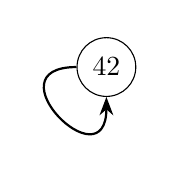
\begin{tikzpicture}
[->/.style={thick,arrows={-Stealth}},
   propG/.style={shape=circle, draw}]
   \path[use as bounding box] (-1, -1) rectangle (0.5, 0.5);
   \node[propG] (P) at (0, 0) {42};
   \draw[->] (P.west) .. controls (-1.5, 0) and (0, -1.5) .. (P.south);
\end{tikzpicture}
\endpgfgraphicnamed
\end{minipage}
\vspace{0.75ex}

\noindent Clearly $m |= 100 |-> 42,100,0$.  But it seems also clear that this memory represents a one-cell cyclic graph as illustrated in the accompanying diagram, \emph{i.e.} we want $m |= \graphkt(100,\hat{\gamma})$, where $\hat{\gamma}(100) = (42,100,0)$.  This is equivalent to wanting to be able to prove $100 |-> 42,100,0 |- \graphkt(100,\hat{\gamma})$.  Unfortunately, as explained in Appendix~C\hide{\ref{apx:problemrecgraph}}, this is rather difficult to do so since applying the natural proof techniques actually strengthens the goal. In fact we do not know if this entailment is provable, but the difficulties encountered in proving what ``should be'' straightforward suggest that Knaster-Tarski should be treated with caution when defining spatial predicates for graphs.

The other direction, \mbox{$\graphkt(100,\hat{\gamma}) |- 100 |-> 42,100,0$},
\textbf{is} true but is not easy to prove, relying on the constructions in \S\ref{sec:goodgraph} and the fact that $\mu_{\mathsf{T}}$ constructs the least fixpoint.  In contrast, $\graphkt(100,\hat{\gamma}) |- 100 |-> 42,100,0 * \top$ is easy. % to prove. % via fold/unfold.

%As explained in~\S\ref{sec:foldunfold}, this alignment is necessary in C-like memory models to prove fold-unfold \eqref{eqn:bigraphintrofoldunfold}, which is why \eqref{eqn:bigraphintrofoldunfold} includes an alignment restriction $x~\mathsf{mod}~16 = 0$ and an existentially-quantified ``blank'' second field for the root $x \mapsto m,-,l,r$.

%As shown in (\ref{eqn:bigraphintrofoldunfold}) of Section
%\ref{sec:orientation}, Hobor and Villard\cite{hobor:ramification}
%defined the separation logic graph predicate
%$\mathsf{graph}(x,\gamma)$ in direct analogy to the standard
%separation logic definition of a tree. Note that the two-neighborhood
%means $\gamma$ is a BiGraph. However, it is peculiarly challenging in
%rigorously formalizing $\p{graph}$.

%* Showing that neither traditional fixpoint method works

%Appel and McAllester proposed another fixpoint $\mu_{\mathsf{A}}$
%that is sometimes used to define recursive predicates in separation
%logic \cite{appel:fixpoint}.  This time the functional $F_P$ needs to be
%\emph{contractive}, which to a first order of approximation means that
%all recursion needs to be guarded by the ``approximation
%modality''~$\rhd$~\cite{appel:vmm}, \emph{i.e.} our graph predicate would
%look like
%\begin{align*}
%\grapham(x, \gamma) ~ &\stackrel{\Delta}{=}\\
% (x = 0 /| \p{emp}) & |/ \exists m,l,r.~ \gamma(x)=(m,l,r) /| \null \\
% x |-> m,l,r & ** \rhd \grapham(l, \gamma) ** \rhd \grapham(r, \gamma)
%\end{align*}
%
%Unfortunately, $\rhd P$ is not precise for all $P$, so $\grapham$ is not precise either.  The approximation modality's universal imprecision has never been noticed before. % in the literature.  %We must do better.

%%%%%%%%%%%%%%%%%%%%%%%%%%%%%%%%%%%%%%%%%%%%%%%%%%
%%%%%% Edit0: cut down contractive recursion
%%%%%%%%%%%%%%%%%%%%%%%%%%%%%%%%%%%%%%%%%%%%%%%%%%


\subsection{Defining a good \p{graph} predicate}\label{sec:goodgraph}

Rather than trying to define \p{graph} as a recursive fixpoint, 
we will instead give it a flat structure.  Graphs in separation
logic have been defined in similar ways before~\cite{ilya-graphs};
our innovation is that we prove---with the amount of precision 
required to convince Coq---that we can still enjoy fold/unfold 
with our flat definition.  Our path starts with the iterated 
separating conjunction or ``big star'', which is first defined over 
lists and then extended to sets as follows:

%%%%%%%%%%%%%%%%%%%%%%%%%%%%%%%%%%%%%%%%%%%%%%%%%%
%%%%%% Edit1
%%%%%%%%%%%%%%%%%%%%%%%%%%%%%%%%%%%%%%%%%%%%%%%%%%
%%%%%% Edit1: Qinxiang's proposal starts
%%%%%%%%%%%%%%%%%%%%%%%%%%%%%%%%%%%%%%%%%%%%%%%%%%
\iftrue
\[
\begin{array}{@{}l@{}}
\underset{\{l_1, l_2,\dots,l_n\}}{\bigstar}P ~~ \defeq ~~ P(l_1) *
  P(l_2) * \dots * P(l_n) \\
\underset{S}{\bigstar} P ~~ \defeq ~~ \exists L.~ (\p{NoDup}\ L) /| (\forall x.~ x\ \p{in}\ L <=> x \in S) /| \underset{L}{\bigstar}P
\end{array}
\]
We are now ready to define a good \p{graph} predicate:
\fi
%%%%%%%%%%%%%%%%%%%%%%%%%%%%%%%%%%%%%%%%%%%%%%%%%%
%%%%%% Edit1: Qinxiang's proposal ends
%%%%%%%%%%%%%%%%%%%%%%%%%%%%%%%%%%%%%%%%%%%%%%%%%%
%%%%%% Edit1: Original version starts
%%%%%%%%%%%%%%%%%%%%%%%%%%%%%%%%%%%%%%%%%%%%%%%%%%
\iffalse
\begin{equation*}
  \underset{\{l_1, l_2,\dots,l_n\}}{\bigstar}P ~~ \defeq ~~ P(l_1) *
  P(l_2) * \dots * P(l_n).
\end{equation*}
Formally $\bigstar$ is defined over a list rather than a set and is parameterized by a predicate $P$.  It is natural to extend $\bigstar$ to a set $S$ with an existentially-quantified duplicate-free list~$L$:
\[
\underset{S}{\bigstar} P ~~ \defeq ~~ \exists L.~ (\p{NoDup}\ L) /| (\forall x.~ x\ \p{in}\ L <=> x \in S) /| \underset{L}{\bigstar}P
\]
We use the same $\bigstar$ notation since the concepts are similar, but the existential adds a little pain since we need to prove that all choices of $L$ yield equivalent predicates.

We are now ready to give a good \p{graph} predicate:
\fi
%%%%%%%%%%%%%%%%%%%%%%%%%%%%%%%%%%%%%%%%%%%%%%%%%%
%%%%%% Edit1: Original version ends
%%%%%%%%%%%%%%%%%%%%%%%%%%%%%%%%%%%%%%%%%%%%%%%%%%
\vspace{-1.5ex}
\begin{equation}\label{eqn:iter_def}
  \p{graph}(x, \gamma) ~~ \defeq ~~ \underset{v \in \mathit{reach}(\gamma, x)}{\bigstar} v\mapsto\gamma(v)
\vspace{-1.5ex}
\end{equation}
$\gamma$ is a GeneralGraph and ``$x |-> \gamma(x)$'' is a predicate that says how a single node fits in memory. In Figure~\ref{fig:markgraph} it was:
\[
\exists m,l,r.~\gamma(x) = (m,l,r) /| x |-> m,-,l,r /| x\ \p{mod}\ 16 = 0
\]
{\color{magenta}$\gamma$ need not be a bigraph, but \emph{e.g.} can have many edges.}

Our definition of \p{graph} is flat in the sense that there is no obvious way to follow the link structure recursively.  Happily, we can recover a general recursive fold/unfold (if $x |-> \gamma(x)$ and the GeneralGraph has the necessary properties in its soundness condition):
\vspace{-1ex}
\begin{equation}
\label{eqn:unfold_graph}
\hspace{-1em}\begin{array}{@{}lc@{\hspace{1pt}}c@{\hspace{1pt}}l@{}}
\p{graph}(x,\gamma)  <=>  x |-> \gamma(x) ** \big(\!\!\!\!\!\!\!\!\!\!\!\!\!\underset{\color{magenta}n \in \p{neighbors}(\gamma,x)}{\raisebox{-0.3ex}{\resizebox{0.75em}{!}{$\scon$}} \hspace{-2.18ex} \bigcup}\!\!\!\!\!\!\!\!\!\!\!\! \p{graph}(\gamma,n) \big) \\
[2pt]
\text{~~~ where ~~ }\underset{l_1,\dots,l_n}{\raisebox{-0.3ex}{\resizebox{0.75em}{!}{$\scon$}}\hspace{-2.18ex} \bigcup} \! \! P  \defeq  P(l_1) ** \ldots ** P(l_n) \end{array}
\vspace{-1ex}
\end{equation}

The proof of the $<=$ direction requires care. The difficulty is that if two nodes $x |-> \gamma(x)$ and $x' |-> \gamma(x')$ are \emph{skewed}, \emph{i.e.} ``partially overlapping'' with some---but not all---of $x$'s memory cells shared with $x'$, then the $\bigstar$ on the left hand side cannot separate them.  To avoid skewing we require that $x |-> \gamma(x)$ be \emph{alignable}. A predicate $P$ is alignable when
\[
\forall x,y.~ \Big(P(x) ** P(y) |- \big(P(x) /| x = y\big) |/ \big(P(x) * P(y)\big)\Big)
\]
That is, they overlap either completely or not at all. In a Java-like memory model this property is automatic because pointers in such a model always point to the root/beginning of an object.  In contrast, in a C-like memory model such as in VST/CompCert, this property is not automatic because pointers can point anywhere.  In such a model, alignment is most easily enforced by storing graph nodes at addresses that are multiples of an appropriate size (16 in Figure~\ref{fig:markgraph}).

{\color{magenta}Some of our VST proofs do not use fold/unfold, instead preferring to use the lemmas in~\S\ref{sec:ramifylib} directly.  On the other hand, for HIP/SLEEK fold/unfold is vital, and it is heartening to know that the recursive relationship holds.  We also prove fold/unfold lemma for DAGs in which we get a $*$ between the root and its $**$-joined neighbors. % rather than the $**$ present in \eqref{eqn:unfold_graph}.
}

\subsection{Ramification Libraries}\label{sec:ramifylib}

\begin{figure}[t]
\centering
\beginpgfgraphicnamed{infrastructure}
\begin{tikzpicture}[
->/.style={thick, arrows={-Stealth}},
ent/.style={shape=rectangle, rounded corners=4pt, draw, on grid}]
\node[ent] (SM) at (0, 0) {\small Step-Indexed Model};
\node[ent] (DM) [right=4.4 of SM] {\small Direct Model};
\node[ent] (CL) [above=1 of SM] {\small Core Logic};
\node[ent] (SL) [above=1 of DM] {\small Supplementary Logic};
\node[ent] (LF) [above left=1 and 1.2 of CL] {\small Logic Facts};
\node[ent] (RF) [above right=1 and 1.2 of CL] {\small Basic Ramification};
\node[ent] (BF) [above=1 of LF] {\small $\bigstar$ Facts};
\node[ent] (BR) [above=1 of RF] {\small $\bigstar$ Ramification};
\node[ent] (GF) [above=1 of BF] {\small Graph Facts};
\node[ent] (GR) [above=1 of BR] {\small Graph Ramification};
\node[ent] (SLF) [above=1 of SL] {\small Supplementary Logic Facts};
\node[ent] (SBF) [above=1 of SLF] {\small Supplementary $\bigstar$ Facts};
\node[ent] (SGF) [above=1 of SBF] {\small Supplementary Graph Facts};
\draw [double, ->] (SM) to (CL);
\draw [double, ->] (SM) to (SL);
\draw [double, ->] (DM) to (CL);
\draw [double, ->] (DM) to (SL);
\draw [->] (CL) to (LF);
\draw [->] (CL) to (RF);
\draw [->] (CL) to (SL);
\draw [->] (SL) to (SLF);
\draw [->] (SLF) to (SBF);
\draw [->] (SBF) to (SGF);
\draw [->] (LF) to (RF);
\draw [->] (LF) to (BF);
\draw [->] (RF) to (SLF);
\draw [->] (RF) to (BR);
\draw [->] (BF) to (BR);
\draw [->] (BF) to (GF);
\draw [->] (GF) to (GR);
\draw [->] (GR) to (SGF);
\draw [->] (BR) to (GR);
\draw [->] (BR) to (SBF);
\node (legend1) [below right=0.2 and -1.2 of SM] {\small Dependence};
\coordinate[left=0.8 of legend1]  (l1);
\draw [->] (l1) to (legend1);
\node (legend2) [right=1 of legend1] {\small Instantialization Choices};
\coordinate[left=0.8 of legend2]  (l2);
\draw [double, ->] (l2) to (legend2);
\end{tikzpicture}
\endpgfgraphicnamed
\vspace{1ex}
\caption{Infrastructure of ramification library}\label{fig:infra}
\end{figure}

We provide the architecture of our spatial development in Figure~\ref{fig:infra}.  Starting from the bottom, notice that there are two underlying heap models: the Step-Indexed Model, which is the main heap model used in VST, and a much simpler Direct Model, {\color{magenta} which is used by HIP/SLEEK among others}. The Step-Indexed model is much fancier, but none of our development depends on its bells and whistles.

To isolate our development from these unnecessary complications, 
{\color{magenta}and to ensure that HIP/SLEEK can reuse our spatial 
reasoning, we use two interfaces: Core Logic and Supplementary 
Logic.  Both models can instantiate both interfaces, but generally 
speaking our VST proofs only need the Core properties to prove 
our examples, whereas HIP/SLEEK uses both Core and Supplemental.} 
Each interface defines some operators of separation logic and 
provides some axioms about how they work.  For example, $*$ and 
$--*$ are in Core Logic, along with the axiom 
$(P |- Q --* R) <=> (P * Q |- R)$.  On the other hand, 
the $**$ and $--o$ operators are in Supplementary Logic, 
along with rules like $P |- P ** P$.

Above the Logic layer we have three towers, each three levels high.  The leftmost tower contains basic lemmas about Logic, $\bigstar$, and \p{graph}.  In the $\bigstar$ Facts box we prove \emph{e.g.}:
\[
\infrule{}
{A \cap B = \emptyset}
{\underset{x\in A}{\bigstar} P(x) \; * \underset{x\in B}{\bigstar} P(x) \;\, \Leftrightarrow \underset{x\in A \cup B}{\bigstar} P(x)}{}
\]

The middle tower is more interesting in that it is entirely focused on ramification entailments.  A robust library of ramification entailments is essential to make ramification work smoothly in practice.  The lowest level contains lemmas like:
\[
%\infrule{Ramify-Q-SPLIT}
\infrule{}
{G_1 \vdash L_1 * \forall x.~ (L_2 --* G_2) \\
 G'_1 \vdash L'_1 * \forall x.~ (L_2' --* G'_2)}
{G_1 * G'_1 \vdash (L_1 * L'_1) * \forall x.~ \big((L_2 * L'_2)--* (G_2 * G'_2)\big)}{}
\]
We use this lemma to break large ramification entailments into more manageable pieces in a compositional way. % compositionally.

The middle level contains $\bigstar$ ramification lemmas, \emph{e.g.}:
\begin{equation}
\label{ramify:bigstar}
\infrule{}
{A \cap B = \emptyset  \qquad  A' \cap B = \emptyset}
{\underset{x\in A\cup B}{\bigstar} P(x) \vdash \! \underset{x\in A}{\bigstar} \! P(x) * \Big( \underset{x\in A'}{\bigstar} \! P(x) \! \wand \! \! \! \! \underset{x\in A' \cup B}{\bigstar} \! \! P(x)\Big)}{}
\end{equation}

The top level is focused on graph ramifications, such as the ``update one node'' lemma:
\begin{equation}
\label{lem:updategraphnode}
%{\gamma(x_0) = \gamma'(x_0) \text{ for any } x_0 \neq x }
\infrule{}
{\forall x_0 \neq x.~ \gamma(x_0) = \gamma'(x_0) \\ \p{neighbors}(\gamma,x)=\p{neighbors}(\gamma',x)}
{\p{graph}(x, \gamma) \! \vdash \! x \! \mapsto \! \gamma(x) \! * \! \big(x \! \mapsto \! \gamma'(x) \! \wand \! \p{graph}(x, \gamma')\big)}{}
\end{equation}
This lemma was used on line~\ref{code:markram2} in Figure~\ref{fig:markgraph}.

This layered structure enables proof reuse. All of the theorems for $\p{graph}$ are proved from the properties of iterated separating conjunction, but having a modular library allows $\bigstar$ to be reused in other structures smoothly.

Also, all of our verifications of different graph algorithms use the proof rules of $\p{graph}$ at the top level in the library. Taking the marking algorithm we introduced in \S\ref{sec:orientation} as an example, we prove the following theorem from the library:
\begin{equation}
\label{lem:updatesubgraph}
\frac
{n \in \p{neighbors}(\gamma,x)}
{
\mbox{
$\begin{array}{@{}l@{}l@{}}
\p{graph}(x, \gamma) \vdash \\
\p{graph}(n, \gamma) \! * \!
\big(\forall \gamma'. \m{mark}(\gamma, n, \gamma') \! /| \! \p{graph}(n, \gamma') \! --*
\m{mark}(\gamma, n, \gamma') \! /| \! \p{graph}(x, \gamma')\big)
\end{array}$
}
}
\end{equation}

The Supplementary tower contains properties not used by most of the VST examples.  This includes the fold/unfold relationship from \S\ref{sec:goodgraph}, facts about precision, \emph{etc}. Some of these properties are needed by HIP/SLEEK, while others are mostly included for completeness.

% are there just because we felt they might be useful in the future.

%One benefit of the definition in (\ref{eqn:iter_def}) is that the pure
%mathematical graph $\gamma$ in $\mathtt{graph}$ is not necessarily a
%BiGraph. (\ref{eqn:iter_def}) can represent a general graph with
%variant number of neighors as long as extending the definition of
%$\gamma(x)$ to data mapped by the label function and every neighbor of
%node $x$.
%
%Moreover, it turns out that the $\bigstar$ notation is a more useful
%and fundamental concept than $\mathtt{graph}$. There are two parts of
%the $\bigstar$ in (\ref{eqn:iter_def}): one is the predicate $\mapsto$
%and the other is the node set which the $\mapsto$ iterates on. They
%both bind to $\gamma$ in (\ref{eqn:iter_def}) for $\p{graph}(x,
%\gamma)$, which is a special case. In section \ref{sec:applicable}, we
%will see the specification of a spanning tree algorithm which uses
%$\bigstar$ directly instead of $\p{graph}$ because in that
%specification, the predicate $\mapsto$ and the node set bind to
%different mathematical graphs. Furthermore, we generalize the
%ramification rules for $\p{graph}$ in \cite{hobor:ramification}, which
%uses $\bigstar$ so as to be applied in all verification examples.

%% 1.2. \texttt{Iter\_sepcon} and \texttt{pred\_sepcon} are defined. And related ramification rules are proved.
%% 1.3. The most general graph-spatial-predicate \texttt{vertices\_at} are defined (for all possible styles of graphs). Related ramification rules are proved. Graph and graphs are defined as special cases of vertices at.

%% 2. A minor implementation trick. There are many tactics defined in \texttt{msl\_ext/ramify\_tactics.v}, which can manipulate low level heaps efficiently.

%% * Separating the material into the general vs. tool-specific part.  Measurements of etc.


\section{Verifying graph-manipulating programs}

4. General Strategy for Verifying Programs
4.1. Using relation. (Better for proof's code reuse). For example, spanning tree is mark together with some structural requirement.
4.2. Using existential quantifier in post condition.

DO WE NEED RAMIFICATION BEFORE THIS SECTION?

VST is a correctness-certified tool to prove functional correctness of C programs CITE. All Hoare rules are proved sound and users can use them to build modularized proof. At the same time, users can have all the convenience offered by separation logic. For example, frame rule is already proved sound as well. VST is fully developed in Coq and it uses the C semantics offered by ComCert. CITE

AQUINAS, IS IT CORRECT TO USE PRESENT TENSE TO TALK ABOUT VST? SHALL I USE PAST TENSE?

$$ \frac{\{ P \} c \{Q \} \quad FreeVar(F) \cap ModVar(c) = \emptyset } {\{P * F \} c \{ Q * F \}} $$

\[
\frac{
\begin{array}{c}
\{ L \} c \{L' \} \quad FreeVar(L' -* G') \cap ModVar(c) = \emptyset \\
G \vdash L * (L' -* G')
\end{array}
}
{\{G \} c \{ G' \}}
\]

EDITING FORMAT

In this work we present, we establish the soundness of ramification rule based on frame rule. Noticing that local variables are stored in stack in C, expressing the property of a local variable's value is a pure fact rather than a spatial fact. So, we prove a pure-facts-related rule besides the primary one such that ramification is much easier to apply in VST.

\[
\frac
{
\begin{array}{c}
\{ L \} c \{PureLocal \wedge L' \} \\ 
FreeVar(PureFrame \wedge (L' -* G')) \cap ModVar(c) = \emptyset \\
G \vdash L * (PureFrame \wedge (L' -* G'))
\end{array}
} {\{G \} c \{ PureFrame \wedge PureLocal \wedge G' \}}
\]

EDITING FORMAT


MORE TO WRITE: divide pure facts into frame and local based on VST's canonical form. Based on localize/unlocalize, compared with frame rule, ramification rule have better use on VST's automatic symbolic execution system.





2.4. VST instance of \texttt{pSpatialGraph\_Graph\_Bi} and \texttt{sSpatialGraph\_Graph\_Bi} are constructed in "\texttt{spatial\_graph\_aligned\_bi\_VST.v}" and "\texttt{spatial\_graph\_unaligned\_bi\_VST.v}".

3. Embed ramification into VST.
3.1. Ramification rule are proved sound in VST.
3.2. A special ramification rule for VST's Sep-Local-Prop style pre/post condition is prove. The point is traditional ramification rule require the whole frame-like-wand-expression to be closed w.r.t. the modified variables. This special rule split closed and unclosed away.
3.3. Localize and unlocalize are defined.
3.3.1. Localize/unlocalize offer a user-friendly way of using ramification rule.
3.3.2. Unlocalize tactic need "Grab Existential Variables" afterwards. It is not nice.
3.3.3. Writing Ocaml plugin is one solution. But we need to develop for both mac and windows.
3.3.4. Or we can see whether Coq's next version offers more tactics for existential variables.


\section{Enabling externally-verified lemmas in HIP/SLEEK}

* the connection to HIP/SLEEK

\section{Applying ramification}

5. Mark algorithm
5.1. For Ramification-Paper-style proof
5.1.1. Math land theorems for marking algorithm (general situation and bi-graph situation) are all proved. Mainly in "\texttt{marked\_graph.v}" and "\texttt{spatial\_graph\_mark\_bi.v}".
5.1.2. Ramification rule for marking algorithm (bi-graph situation) are all proved in "\texttt{spatial\_graph\_mark\_bi.v}".
5.1.3. Combining 2.4 and 3.1.1 and 3.1.2, we have a end-to-end proof for marking-graph in VST.
5.1.4. We have an end-to-end proof for marking-dag, but not defining dag predicate as a whole.
5.1.5. The module type which will be generated by HIP/SLEEK should be instantiated by 2.2 and 2.5.

6. Spanning tree algorithm
6.1. We divide the spanning tree relation into structural part and marking part. They are both defined properly.
6.2. Important pure facts and ramification rules are not proved yet.
6.3. Shengyi has already known how to use VST to handle the C program of bigraph spanning tree.

\section{Related and future work}

5.2. An alternative way of verifying marking program is reasoning about the whole history of marking operations. The disadvantage of it is that it currently needs more work in a Hoare logic framework. The advantage of it is that its reasoning structure are more similar with the way we understand it in our first algorithm class.
5.3. I take some effort on garbage collector like graph structural. Though it is only connecting this special structural with 5.1.1 and 1.3, it takes much time and it is not finished yet.

\section{Conclusion}

\bibliographystyle{abbrvnat}
\bibliography{autoquack}

\end{document}
